\subsection{Performance Evaluation}\label{sec:cloud:virtualized_network_functions:performance_evaluation}

We implement the models introduced in \refsec{sec:cloud:virtualized_network_functions:model} using a \gls{DES} with the SimPy~\cite{SimPy2015} package as foundation.
The implementation\footnote{\url{https://github.com/fmetzger/ggsn-simulation/}} as well as the considered scenarios\footnote{\url{https://github.com/cschwartz/ggsn-simulation-studies/}} are also publicly available as a reference.
To be in line with the measurement data we consider a simulation time for all simulation scenarios of 7 days, with a transient phase of 60 minutes.
Ten replications of each scenario were performed.
All error bars given in this section show the \SIrange{5}{95}{\percent} quantiles of all replications.

We use the measurements introduced in \refsec{sec:cloud:virtualized_network_functions:measurement_data} in order to dimension a traditional \gls{GGSN} as a baseline for all further studies.
Based on these results, we first examine the effects of network function virtualisation by scaling \emph{out} instead of up through a virtual \gls{GGSN} model.
Finally, we arrive at a more realistic version of the virtual \gls{GGSN} by taking the start up and shut down times into account.

\subsubsection*{Traditional \headershortacr{GGSN}}\label{sec:cloud:virtualized_network_functions:performance_evaluation:traditional_ggsn}

Employing the inter-arrival times and duration of tunnels, we first study the traditional \gls{GGSN} model introduced previously.
Whilst our measurements provide us with information on the frequency of new tunnels and the duration they remain active, we have no reliable information on the number of active tunnels the \gls{GGSN} can support.
Thus, in a first step, we dimension the \gls{GGSN} in such a way that a suitable blocking probability \(\blockingprobability\) can be achieved.

%TODO grafik? traditional-blocking + text?

In order to obtain a baseline dimensioning, we perform a simulation study, considering the impact of an increasing offered load on the blocking probability.
We observe that as the number of supported parallel tunnels increases, the blocking probability decreases.
For the normalized inter-arrival no blocking is occurring if we allow for more than \(5000\) parallel tunnels.
Thus, we consider the range of \(4000\) to \(5000\) parallel tunnels to be of special interest for the remainder of the study.

\subsubsection*{Virtual \headershortacr{GGSN}}\label{sec:cloud:virtualized_network_functions:performance_evaluation:virtual_ggsn}

In order to study the feasibility of the virtual \gls{GGSN} approach discussed in \refsec{sec:cloud:virtualized_network_functions:model}, we compare the performance metrics of the virtual \gls{GGSN} with that of a traditional \gls{GGSN}.
To this end, the virtual \gls{GGSN} is simulated in varying configurations.
The number of servers and supported tunnels per server is chosen in such a way that the results can be compared with those obtained from our study of the traditional \gls{GGSN}.
Due to simulation time constraints, only a representative subset of scenarios is simulated.

In the virtual \gls{GGSN} model, servers are activated and deactivated on demand, while in the traditional \gls{GGSN} model, the single server is always on.
For this investigation a conservative start up and shut down time of \SI{300}{\second} is chosen.
Generally, deactivating server instances reduces energy consumption and frees up inactive servers for other use.
For this reason, the number of active servers is a relevant performance metric in the virtual \gls{GGSN} model.

\begin{table}\caption{Manipulation check for the experimental factors based on one-way ANOVA.}
\centering
\label{tab:cloud:virtualized_network_functions:performance_evaluation:virtual_ggsn:manipulation}
\tabcolsep=0.11cm
\begin{tabular}{lccccc}
\toprule
& \(F(2,1275)\) & \(\eta^2_p\) & \(p\) & Cohen's & Cohen's\\ 
&  & & & \(f^2\) & \(\hat{\omega}^2\) \\ 
\midrule
\emph{blocking probability} \(\blockingprobability\)  & & & & &\\ 
maxTunnels \(n\)&  15601.53 & \textcolor{orange}{0.993} & $<0.001$ & \textcolor{orange}{26.73} & 0.96\\ 
maxInstances \(\maxServers\)&  10218.17 & \textcolor{orange}{0.986} & $<0.001$ & \textcolor{orange}{1.06} & 0.51\\ 
startstopDuration &  0.86 & \textcolor{black}{0.003} & $0.482$ & \textcolor{black}{0.00} & 0.00\\ 
\midrule
\emph{mean tunnel count}  & & & & &\\ 
maxTunnels \(n\)&  20448.34 & \textcolor{orange}{0.994} & $<0.001$ & \textcolor{orange}{27.71} & 0.96\\ 
maxInstances \(\maxServers\)&  13348.25 & \textcolor{orange}{0.989} & $<0.001$ & \textcolor{orange}{1.06} & 0.51\\ 
startstopDuration &  2.87 & \textcolor{black}{0.009} & $0.022$ & \textcolor{black}{0.00} & 0.00\\ 
\bottomrule
\end{tabular}
\end{table}

In order to analyse the influence of the different model parameters on the performance metrics, we perform a one-way ANOVA analysis with the results in \reftab{tab:cloud:virtualized_network_functions:performance_evaluation:virtual_ggsn:manipulation}.
High values for \(\eta_p^2\) and Cohen's \(f^2\)\cite{Ellis2010} indicate that the main influence for both blocking probability \(\blockingprobability\) and mean number of tunnels is the maximum number of tunnels \(n\) and virtual \gls{GGSN} instances \(\maxServers\), i.e. the total number of possible concurrent tunnels in the system.
Therefore, we study these parameters first.

\begin{figure}
  \centering
  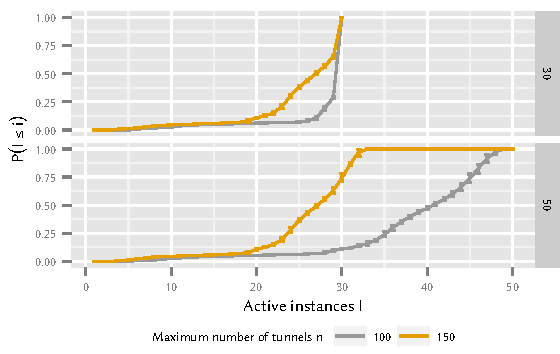
\includegraphics{cloud/virtualized_network_functions/performance_evaluation/figures/instanceuse_multiserver}
  \caption{Impact of the maximum number of tunnels and number of servers on number of active servers in the virtual \headershortacr{GGSN} model.}
  \label{fig:cloud:virtualized_network_functions:performance_evaluation:virtual_ggsn:instanceuse_multiserver}
\end{figure}

In \reffig{fig:cloud:virtualized_network_functions:performance_evaluation:virtual_ggsn:instanceuse_multiserver} the \gls{CDF} of the number of active servers for four different virtual \gls{GGSN} configurations is displayed.
First, we study the behaviour of a virtual \gls{GGSN} with \(30\) servers, where each server can support \(100\) or \(150\) tunnels.  
We compare this with a virtual \gls{GGSN} with \(50\) servers and again \(75\) or \(150\) tunnels.
We observe that increasing the number of supported tunnels per server allows a larger percentage of servers to be shutdown or used for other tasks. This demonstrates the scaling capability of the virtualised model quite well.
Note that both the scenario with \(30\) servers and \(150\) maximum tunnels per server as well as the scenario with \(60\) servers and \(75\) maximum tunnels per server share the same maximum amount of tunnels, i.e. \(4500\), being right at the centre of the interesting range of candidates.

\begin{figure}
  \centering
  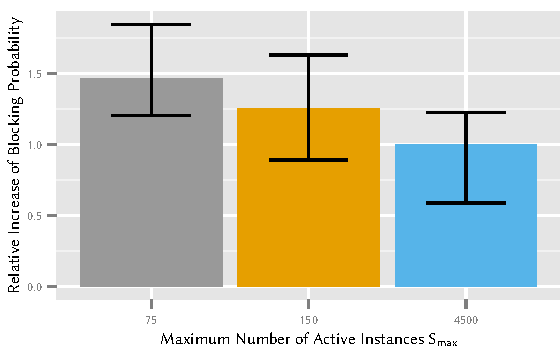
\includegraphics{cloud/virtualized_network_functions/performance_evaluation/figures/blocking_comparison}
  \caption{Impact of blocking probability on the number of servers compared to the traditional \headershortacr{GGSN}, \(4500\) maximum tunnels per server being on a single server, i.e. \(150\) on \(30\), and \(75\) on \(60\) servers.}
  \label{fig:cloud:virtualized_network_functions:performance_evaluation:virtual_ggsn:blocking_comparison}
\end{figure}

Next, we study the blocking probability of the virtual \gls{GGSN} system in \reffig{fig:cloud:virtualized_network_functions:performance_evaluation:virtual_ggsn:blocking_comparison} and compare it to the results from the traditional \gls{GGSN} model with both systems dimensioned for \(4500\) tunnels.
We observe that, considering the start up and shut down time of \SI{300}{\second}, the blocking probability increases by a factor of \(1.46\) if the the virtual \gls{GGSN} is comprised of \(60\) instances dimensioned for \(75\) concurrent tunnels, i.e. \(\frac{1}{60}\) of the original server capacity.
In this case \(27\) of all \(60\) servers can be turned off or used for other purposes at \SI{50}{\percent} of the time.
We conclude that choosing more powerful servers decreases the blocking probability but reduces the potential to disable servers.

So far we have considered a conservative start up and shut down time of servers of 5 minutes, which can potentially occur if current generation physical servers are used.
In the next section we study the impact of reduced start up and shut down times with modern servers with fast storage, e.g. \glspl{SSD}, or containerised applications.

\subsubsection*{Impact of Startup and Shutdown Times}\label{sec:cloud_virtualized_network_functions:startup_shutdown}

In this section, we first consider the impact of different boot and shut down times on resource utilisation and blocking probabilities.
Afterwards, the influence of varying server start and stop times on a fixed combination of maximum tunnels and servers in the system is examined.

\begin{figure}
  \centering
  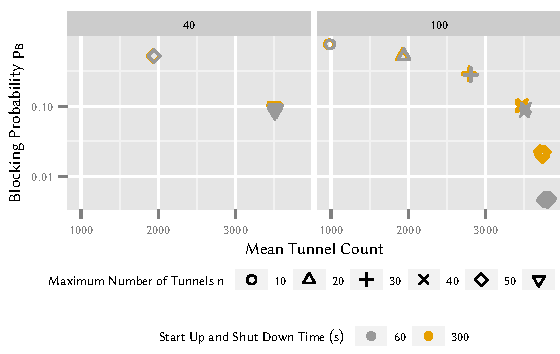
\includegraphics{cloud/virtualized_network_functions/performance_evaluation/figures/compare_util_block}
  \caption{Trade-off between blocking probability and mean resource utilisation with regard to maximum number of instances, maximum number of tunnels per server, and start up and shut down time.}
  \label{fig:cloud_virtualized_network_functions:startup_shutdown:compare_util_block}
\end{figure}

\reffig{fig:cloud_virtualized_network_functions:startup_shutdown:compare_util_block} shows scenarios with \(40\) and \(100\) number of virtual \gls{GGSN} instances and  \(1000\) to \(5000\) total concurrent tunnels.
For each scenario, we study the impact of selecting a different maximum number of tunnels per server as well as start up and shut down times on blocking probability and mean resource utilisation.
The first observation is that by increasing the number of servers, i.e. scaling out, the blocking probability can be decreased, while maintaining a relatively low mean resource utilisation.
In addition to the previous effects, we notice that a higher start up and shut down time causes a slight increase in blocking probability for servers with low tunnel capacity.

\begin{figure}
  \centering
  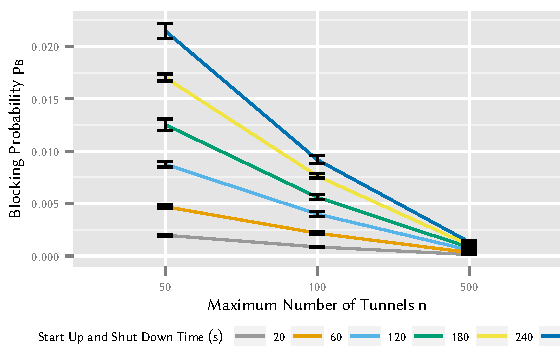
\includegraphics{cloud/virtualized_network_functions/performance_evaluation/figures/compare_maxinstances_block}
  \caption{Influence of start up and shut down time on blocking probability with regard to different numbers of servers.}
  \label{fig:cloud_virtualized_network_functions:startup_shutdown:compare_maxinstances_block}
\end{figure}
 
In order to study this behaviour in more detail, we focus on a specific scenario in \reffig{fig:cloud_virtualized_network_functions:startup_shutdown:compare_maxinstances_block}, where \(5000\) total tunnels should be supported by the system.
In order to achieve this goal, we consider three types of instances, with the server capacity varying between \(50\) and \(500\).
In each case we change the start up and shut down time between \SIrange{20}{300}{\second}.
We observe that lower server capacities combined with higher start up and shut down times increase the blocking probability.
This is due to the server start up threshold mechanism, used in the model, not taking the additional capacity gained by activating an additional server into account.
If a low capacity server with a long boot time is activated, there is a high probability that the system will quickly expend its capacity again.

Thus, it can be concluded that if smaller instances are to be used, for example due to the fact that they are cheaper than large instances, start up and shut down times should be kept minimal, for example by using containers or \glspl{SSD}.